% !TeX root = ../../tesis.tex

% =============================================================================
%  4.2.4 — CONSTRUCCIÓN DEL GRAFO
% =============================================================================
\section{Construcción del Grafo Topológico}
\label{sec:vft-grafo}

\subsection{De la Geometría GeoJSON a NetworkX}
\label{subsec:vft-geom-networkx}

El módulo central del sistema es la clase \texttt{\textbf{VFTGraphBuilder}}
\allowbreak{} (\path{src/core/services/graph_builder.py}), responsable de
transformar las geometrías \geojson{} en un \textbf{dígrafo} representado
mediante la biblioteca \textbf{NetworkX} de Python \citep{hagberg2008networkx}.
La construcción opera en dos fases internas:

\begin{description}
    \item[\textbf{Fase 1 — Registro de estaciones (nodos):}]
    Cada estación del \geojson{} se convierte en un nodo del grafo,
    identificado por sus coordenadas geográficas (longitud, latitud) y
    enriquecido con sus atributos operativos: nombre, sistema de transporte,
    jerarquía, alcaldía y condición de nodo \textsc{cetram}.

    \item[\textbf{Fase 2 — Trazado de rutas (aristas):}]
    Para cada ruta del \geojson{}, el constructor recorre el
    \texttt{MultiLineString} segmento a segmento, acumulando distancia y
    detectando qué estaciones se encuentran sobre el trazo mediante una
    estructura de búsqueda espacial (\termino{KDTree}) con una tolerancia de
    50~m. Por cada par de estaciones consecutivas detectadas, crea una arista
    con la distancia real acumulada a lo largo del trazo —no la distancia en
    línea recta entre las estaciones—. Esta distinción es crítica para sistemas
    como \textsc{rtp} y Corredores Concesionados, cuyos trazos urbanos pueden
    ser hasta un 40~\% más largos que la cuerda directa.
\end{description}
\subsection{Snapping Lógico Geográfico}
\label{subsec:vft-snapping}

En el modo de integración realista (\texttt{REALISTIC\_INTEGRATION}), el
constructor agrega aristas adicionales de \textbf{transbordo peatonal} entre
estaciones de distintos sistemas que se encuentran dentro de una distancia
configurable. Este proceso —denominado \termino{Snapping Lógico Geográfico}—
representa el comportamiento real del pasajero, que puede caminar de una
estación a otra aunque no estén formalmente conectadas en los datos oficiales.

% --- BLOQUE DE IMÁGENES DEL PROCESO DE SNAPPING ---
\begin{figure}[H]
    \centering
    \begin{subfigure}[b]{0.32\textwidth}
        \centering
        \includegraphics[width=\textwidth]{Figures/Cap4/SnappingProcess1.png}
        \caption{Nodos aislados}
        \label{fig:snap1}
    \end{subfigure}
    \hfill
    \begin{subfigure}[b]{0.32\textwidth}
        \centering
        \includegraphics[width=\textwidth]{Figures/Cap4/SnappingProcess2.png}
        \caption{Evaluación de umbral}
        \label{fig:snap2}
    \end{subfigure}
    \hfill
    \begin{subfigure}[b]{0.32\textwidth}
        \centering
        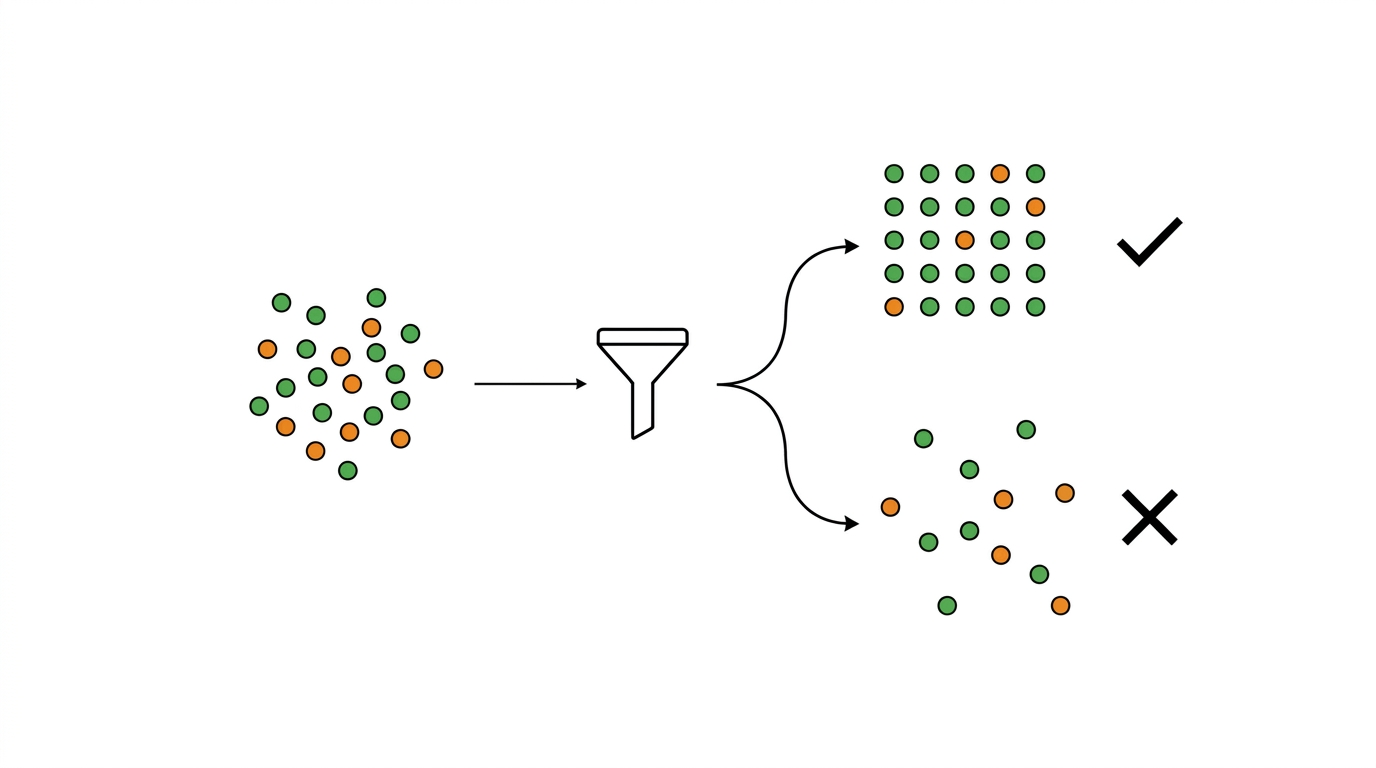
\includegraphics[width=\textwidth]{Figures/Cap4/SnappingProcess3.png}
        \caption{Arista de transbordo}
        \label{fig:snap3}
    \end{subfigure}
    \caption[Secuencia del Snapping Lógico Geográfico]
{Representación visual del proceso de \termino{Snapping Lógico Geográfico}. Las
estaciones
cercanas de distintos sistemas se conectan mediante aristas de transbordo si
cumplen con
    la tolerancia de distancia establecida.}
    \label{fig:proceso-snapping}
    \fuentefigura{Elaboración propia (VFTModel, 2026).}
\end{figure}
% --------------------------------------------------

La tolerancia de transbordo se selecciona a partir de seis umbrales estadísticos
derivados del análisis de las distancias reales entre estaciones de la red
metropolitana, definidos bajo la constante \texttt{STATISTICAL\_THRESHOLDS} en
\texttt{src/core/services/graph\_builder.py}.

\begin{table}[H]
    \centering
    \caption[Umbrales estadísticos de transbordo peatonal en VFTModel]{Umbrales
    estadísticos de tolerancia para el \termino{Snapping Lógico Geográfico}.
El umbral \texttt{Q1} (85~m) es el recomendado para integración conservadora;
    \texttt{Q2} (180~m) integra la mayoría de los \textsc{cetram}s formales.}
    \label{tab:vft-umbrales}
    \begin{tabularx}{\textwidth}{|l|r|X|}
        \hline
        \textbf{Clave} & \textbf{Distancia (m)} & \textbf{Interpretación} \\
        \hline
        \texttt{MIN}  &  15 & Mismo recinto arquitectónico \\
        \texttt{Q1}   &  85 & Transbordo rápido y directo (integración conservadora) \\
        \texttt{Q2}   & 180 & Transbordo promedio real; integra la mayoría de \textsc{cetram}s \\
        \texttt{MEAN} & 245 & Promedio matemático (sesgado por valores atípicos) \\
        \texttt{Q3}   & 420 & Límite máximo de caminata forzada aceptable \\
        \texttt{MAX}  & 880 & Caso atípico; posible falso transbordo \\
        \hline
    \end{tabularx}
    \fuentefigura{Elaboración propia con base en \texttt{graph\_builder.py}
    (VFTModel, 2026).}
\end{table}

El grafo de la \zmvm{} en configuración
\texttt{REALISTIC\_\allowbreak{}INTEGRATION Q1} resultante contiene
\textbf{11{,}115 nodos topológicos} y \textbf{45{,}679 aristas} —25{,}197 de
tránsito y 20{,}482 de transbordo peatonal generadas algorítmicamente—, tras
eliminar 1{,}562 aristas que superaron el umbral de falsa conexión de 5~km.

Los registros de construcción completos de la corrida del 2026-04-18, que
documentan cada fase del proceso, se presentan en el Anexo~\ref{anx:vft-codigo}.

\subsection{Modos de Operación}
\label{subsec:vft-modos}

\texttt{VFTGraphBuilder} ofrece dos modos de construcción del grafo, que
determinan si se generan o no las aristas de transbordo peatonal:

\begin{description}
    \item[\texttt{STRICT\_TOPOLOGY}:]
    Construye el grafo matemático puro: únicamente las aristas de tránsito
    definidas explícitamente por las rutas del \geojson{}. No agrega conexiones
    entre sistemas distintos. Útil para analizar la topología interna de cada
    línea en aislamiento o para verificar que el grafo refleja exactamente los
    trazos geográficos.

    \item[\texttt{REALISTIC\_INTEGRATION}:]
    Además de las aristas de tránsito, genera las aristas de transbordo peatonal
    entre estaciones próximas de distintos sistemas. El costo de cada arista de
    transbordo incluye el tiempo de caminata (a 5~km/h, límite superior del
    \citep{sedatu2019manual}) más la espera promedio del siguiente servicio
    ($F_v / 2$). Este modo es el utilizado en todos los cálculos de indicadores
    presentados en el Capítulo~\ref{ch:resultados-vft}.
\end{description}
